\noindent
When dealing with big data sets one of the challenges is to identify significant features. Depending on the data set itself some dimensions might be redundant. Depending on the field of interest some dimensions might not be relevant. To reduce the total number of dimensions and therefore handle large data sets more efficiently PCA is one possible approach. Another one is to design and implement specialized computing units, e.~g. a quantum computing module to solve the feature extraction. Both approaches can be combined to implement a quantum based PCA which has been researched actively already. This section discusses briefly the core concepts of the classical PCA, how to integrate a quantum module into a larger classical context, and the two concepts used in this paper to implement a quantum based PCA.

\subsection{Principal Component Analysis}
\label{subsec:pca}
The algorithm can be used on high-dimensional data to extract the $n$ most significant features and reduce the total number of dimensions and therefore the complexity of a given data set. In their paper \enquote{A Tutorial on Principal Component Analysis} \cite{Shlen_2014} the author gave the example of measuring the motion of an ideal spring: \enquote{This system consists of a ball of mass m attached to a massless, frictionless spring. [...] Because the spring is ideal, it oscillates indefinitely along the $x$-axis [...]. This is a standard problem in physics in which the motion along the $x$ direction is solved by an explicit function of time.} \cite[p. 1]{Shlen_2014} A possible setup of this example measurement can be seen in Figure ~\ref{fig:pcaexample}. As the author addresses, in this simple example three dimensions will be measured although only one dimension is relevant. PCA can be used to identify significant dimensions, in the given example it is the $x$ direction.

\begin{figure}
  \centering
  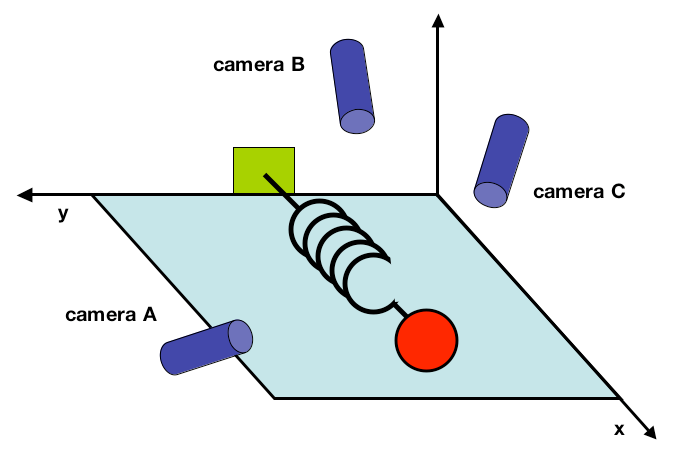
\includegraphics[width=\linewidth]{assets/context_pca_example.png}
  \caption{A simple example of measuring an ideal spring. Figure taken from \cite{Shlen_2014}.}
  \label{fig:pcaexample}
\end{figure}

Let $X$ be an arbitrary data set, represented as an $m \times n$ matrix, with $m$ the number of measurements and $n$ the number of samples. Two very common used techniques are \emph{eigenvector decomposition} or \emph{singular value decomposition}. The eigenvector decomposition leverages the fact that principal components are orthogonal. The approach can be summarized as follows: \enquote{Find some orthonormal matrix $P$ in $Y = PX$ such that $C_Y \equiv \frac{1}{n} YY^T$ is a diagonal matrix. The rows of $P$ are the principal components of $X$.} \cite[p. 6]{Shlen_2014} The singular value decomposition is considered to be a more general solution. It leverages the algebraic concept of change of basis. In this case \emph{any} $X$ can be decomposed as orthogonal matrix $U$, a diagonal matrix $\Sigma$ and another orthogonal matrix $V$ with $X = U\Sigma V^T$. \cite[p. 7]{Shlen_2014}

\subsection{Integration}
\label{subsec:integration}
As for today the actual amount of qubits and therefore the total computing power of quantum devices is limited. Therefore, instead of going for a fully quantum based solution a hybrid architecture that integrates quantum modules into a classical solution often is proposed. This implies two steps of integration, classical pre-processing to encode information into a quantum state and classical post-processing to extract information from a quantum state.

With respect to single qubit quantum state initialization the following solutions can be applied:
\begin{description}
  \item [Zero $|0\rangle$] this is the default state
  \item [One $|1\rangle$] the $X$-Gate, $X = \begin{bmatrix}0 & 1 \\ 1 & 0\end{bmatrix}$ is applied
  \item [Superposition] the $H$-Gate, $H = \frac{1}{\sqrt{2}}\begin{bmatrix}1 & 1 \\ -1 & 1\end{bmatrix}$ is applied
  \item [Amplitude] the $R_y$-Gate, $R_y = \begin{bmatrix}\cos(\frac{\theta}{2}) & -\sin(\frac{\theta}{2}) \\ \sin(\frac{\theta}{2}) & \cos(\frac{\theta}{2})\end{bmatrix}$ can be applied
\end{description}

With respect to multiple qubits quantum state initialization the following solutions can be applied:
\begin{description}
  \item[Classical Register / Bit-wise] The idea is to describe a classical state as a bit string of length $n$ and use register of $n$ qubits to represent it as quantum state. These types of states are straightforward to implement and to measure. The limitations are that a large amount of qubits might be needed resulting into additional hardware limitations and circuit complexity. In their paper \enquote{Loading Classical Data into a Quantum Computer} \cite{Corte_2018} Cortese and Braje proposed a couple of circuit families to address these limitations and to lower the number of qubits needed to represent a classical state as a quantum state up to $O(\log_2{N})$ \cite[p. 35]{Corte_2018} with $N$ being the initial number of qubits used to initialize the circuit.

  \item[State Purification \& Schmidt decomposition] The idea is to describe a classical state as a \emph{pure} or \emph{mixed} quantum state via density operation $\rho$. This operation is defined as $\rho = \Sigma_{i=1}^N p_i| \phi_i \rangle \langle \phi_i |$, $N$ being the number of qubits to be used and $p_i$ the probability for the quantum state to be in the base state $\phi_i$. In case of a pure state this reduces to $\rho = \Sigma_{i=1}^N 1| \phi \rangle \langle \phi |$. The concept of \emph{reduced density operation} leverages the fact that any mixed state $A$ can be enhanced to a larger system and this composed system $AB$ then to be in a pure state. \cite[pp. 98-109]{Niels_2010}\cite[p. 63]{Lokho_2020}\cite{Qtb_Densit} For example, a one-qubit mixed state can be represented as a two-qubits pure state still respecting certain features of the original state being encoded in one of the qubits that are part of the combined (entangled) state. These insights then can be applied to compute an unitary preparation operation $U_{prep}$ for this combined state using \emph{Schmidt decomposition}.\cite[pp. 109-111]{Niels_2010} An entangled quantum state can then be prepared by $U_{prep} = (U_A \otimes U_B) CNOT_{AB} (U_A^{'} \otimes I_B)$, $I$ being the identity operation. \cite[pp. 79-81]{Lokho_2020}

  \item[Amplitude Amplification] The idea is to \enquote{search} for a quantum state via the Grover algorithm. This technique provides the opportunity to initialize a quantum state without explicitly encoding the exact state. \cite[pp.3-4]{Daski_2015}\cite{Qtb_Grover} This method was researched further by Jensen et.~al. and discussed in their paper \enquote{Quantum Computation of Eigenvalues within Target Intervals}. \cite{Jense_2020}
\end{description}

With respect to extracting data from a quantum circuit measurements are used. Interpreting the measurements is done during the classical post-processing. This step is tied close to the problem solved by a quantum solution and involves the following two aspects: (1) find and apply a measurement scheme to extract meaningful information and (2) to be able to handle a certain degree of uncertainty. \cite[p. 5]{Daski_2015}\cite{Qtb_Measu}

\subsection{Quantum based PCA}
\label{subsec:qpca}
In this paper two simplified quantum based PCA algorithms will be explored. Both of them have the general outline:
\begin{itemize}
  \item classical pre-processing: to calculate all relevant unitary operations
  \item quantum state initialization
  \item algorithm specific quantum step
  \item classical post-processing: extract / compute the eigenvalues
\end{itemize}

\begin{figure}
  \centering
  \includegraphics[width=\linewidth]{assets/background_swap_test.png}
  \caption{Swap Test. Figure taken from \cite{Wp_Swap_File}.}
  \label{fig:swap_test}
\end{figure}

\begin{figure}
  \centering
  \includegraphics[width=\linewidth]{assets/background_qpe.png}
  \caption{Quantum Phase Estimation. Figure taken from \cite{Wp_QPE_File}.}
  \label{fig:qpe}
\end{figure}

\begin{description}
\item[Swap test based] The \emph{Swap Test} is an operation to check the level of difference of two quantum states. It takes two quantum states as input, each represented by $n$ qubits. It outputs the level of equality of the two states: (1) if both states are orthogonal to each other the probability to measure $0$ is $\frac{1}{2}$ or (2) if both states are equal to each other the probability to measure $0$ is $1$. This paper followed the algorithm proposed on the respective article on \emph{Wikipedia}. \cite{Wp_Swap} The general outline of the algorithm can be seen in Figure ~\ref{fig:swap_test}.

The algorithm proposed by \cite[pp. 63-66]{Lokho_2020} uses the swap test to compare two states and then the eigenvalues are calculated during post-processing. They proposed the following formula to calculate the two eigenvalues with purity $P = Tr(\rho^2)$, $\rho$ being the density operation:
\begin{itemize}
  \item $e_1 = Tr(\Sigma) \ast (1 + \sqrt{1 - 2 (1 - P)}) / 2$
  \item $e_2 = Tr(\Sigma) \ast (1 - \sqrt{1 - 2 (1 - P)}) / 2$
\end{itemize}

The authors stated that their solution is limited to work on $2 \times 2$ feature matrices. Which is the main reason to refactor the overall solution in a second step and to use QPE for the eigenvalue calculation.

\item[Quantum Phase Estimation] The qiskit textbook states that the \enquote{objective of the algorithm is the following: Given a unitary operator $U$, the algorithm estimates $\theta$ in $U|\psi\rangle = e^{2\pi i\theta}|\psi\rangle$. Here $|\psi\rangle$ is an eigenvector and $e^{2\psi i\theta}$ is the corresponding eigenvalue.}\cite{Qtb_Qpe} The general outline of the algorithm can be seen in Figure ~\ref{fig:qpe}.

The QPE is not limited to work on $2 \times 2$ feature matrices. But the QPE expects the eigenvectors of the feature matrix as the initial quantum state. Furthermore, the additional unitary operation $U$ has to be computed during pre-processing.
\end{description}

